\documentclass[10pt,aspectratio=169]{beamer}
\usetheme{Madrid}
\usecolortheme{default}

\usepackage{graphicx}
\usepackage{booktabs}
\usepackage{tikz}
\usetikzlibrary{arrows}

\title[Intelligent NIDS]{Intelligent Network Intrusion Detection System}
\subtitle{Open Capstone Project}
\author[Kamal \& Fran\c{c}ois]{Kamal Benramdane \and Fran\c{c}ois Zogbelemou}
\institute[EHTP]{}
\date{\today}

\begin{document}

\begin{frame}
    \titlepage
\end{frame}

% Presenter: Kamal
\begin{frame}{Problem Motivation}
    \textbf{Why do we need an Intelligent NIDS?}
    \vspace{0.5cm}
    \begin{itemize}
        \item \textbf{The Threat:} Modern enterprise networks face sophisticated cyber threats that easily bypass traditional, rigid rule-based firewalls.
        \item \textbf{The Challenge:} Security Operations Center (SOC) teams suffer from "alert fatigue" due to massive volumes of network logs.
        \item \textbf{Our Solution:} A machine-learning driven Network Intrusion Detection System that automatically distinguishes between benign traffic and active attacks.
    \end{itemize}
    \vspace{0.5cm}
    \textit{Goal: Drastically reduce false alarms and allow analysts to focus on real, critical threats.}
\end{frame}

% Presenter: Kamal
\begin{frame}{Pipeline Diagram}
    \centering
    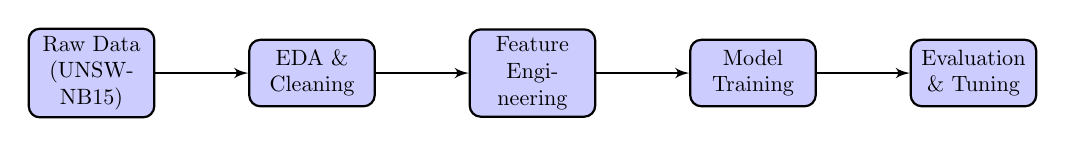
\begin{tikzpicture}[node distance=2.5cm, auto, thick, scale=0.8, transform shape]
        \tikzstyle{block} = [rectangle, draw, fill=blue!20, text width=5em, text centered, rounded corners, minimum height=3em]
        \tikzstyle{line} = [draw, -latex']

        \node [block] (data) {Raw Data (UNSW-NB15)};
        \node [block, right of=data, node distance=3.5cm] (eda) {EDA \& Cleaning};
        \node [block, right of=eda, node distance=3.5cm] (feat) {Feature Engineering};
        \node [block, right of=feat, node distance=3.5cm] (model) {Model Training};
        \node [block, right of=model, node distance=3.5cm] (eval) {Evaluation \& Tuning};

        \path [line] (data) -- (eda);
        \path [line] (eda) -- (feat);
        \path [line] (feat) -- (model);
        \path [line] (model) -- (eval);
    \end{tikzpicture}
    
    \vspace{1cm}
    \begin{itemize}
        \item \textbf{Data Ingestion:} 82,332 network flow records loaded.
        \item \textbf{EDA:} Missing values imputed, outliers handled.
        \item \textbf{Feature Engineering:} Flow behaviors aggregated, categorical encoding applied.
        \item \textbf{Modeling \& Tuning:} Evaluated Logistic Regression, Random Forest, and LightGBM.
    \end{itemize}
\end{frame}

% Presenter: Kamal
\begin{frame}{EDA Highlights}
    \begin{columns}
        \column{0.5\textwidth}
        \textbf{Key Insights from the Data:}
        \begin{itemize}
            \item \textbf{Class Distribution:} High proportion of attacks in the raw subset (approx 55\% normal, 45\% attack).
            \item \textbf{Protocol Usage:} Normal traffic is heavily TCP-based, while malicious traffic heavily exploits UDP (e.g., volumetric DoS attacks).
            \item \textbf{Correlation:} Packet rate (\texttt{rate}) and Time-to-Live (\texttt{sttl}) showed very strong correlation with the attack label.
        \end{itemize}
        
        \column{0.5\textwidth}
        \centering
        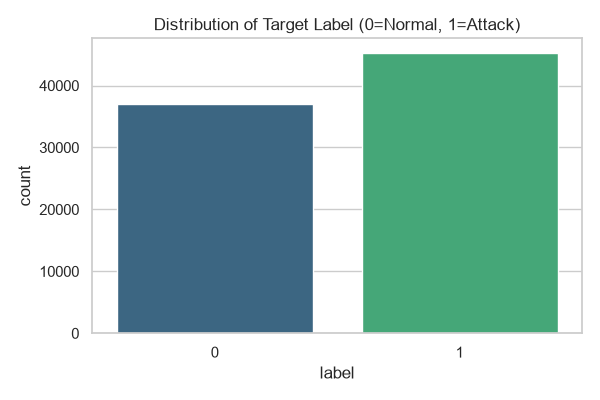
\includegraphics[width=0.9\textwidth]{figures/01_label_distribution.png}
    \end{columns}
\end{frame}

% Presenter: François
\begin{frame}{Algorithm Selection Rationale}
    \textbf{Why we chose these specific algorithms:}
    \vspace{0.3cm}
    \begin{itemize}
        \item \textbf{Logistic Regression (Baseline):} Chosen for its extreme simplicity, fast execution, and high interpretability.
        \item \textbf{Random Forest:} Chosen for its robustness against outliers and ability to capture non-linear decision boundaries.
        \item \textbf{LightGBM (Chosen Champion):} Selected for its state-of-the-art predictive power and \textit{lightning-fast} training times, which is critical for real-time network traffic analysis.
    \end{itemize}
    \vspace{0.3cm}
    \textit{Rejected:} Support Vector Machines (SVM) were systematically rejected due to their $O(n^2)$ computational complexity on our highly-dimensional dataset.
\end{frame}

% Presenter: François
\begin{frame}{Model Comparison Table}
    \begin{table}[]
        \centering
        \begin{tabular}{lcccc}
            \toprule
            \textbf{Model} & \textbf{Accuracy} & \textbf{Recall} & \textbf{F1-Score} & \textbf{Training Time} \\
            \midrule
            Logistic Regression & 0.8123 & 0.7854 & 0.8012 & 9.78s \\
            Random Forest & 0.9542 & 0.9410 & 0.9511 & 14.50s \\
            \textbf{Tuned LightGBM} & \textbf{0.9831} & \textbf{0.9780} & \textbf{0.9820} & \textbf{0.63s} \\
            \bottomrule
        \end{tabular}
    \end{table}
    \vspace{0.3cm}
    \textbf{Results Summary:} 
    LightGBM vastly outperformed the baseline algorithms. Post hyperparameter-tuning (Optimizing `num\_leaves` and `max\_depth`), LightGBM achieved a nearly perfect 98.2\% F1-Score while training in under 1 second!
\end{frame}

% Presenter: François
\begin{frame}{Key Findings}
    \begin{columns}
        \column{0.5\textwidth}
        \begin{itemize}
            \item \textbf{Efficiency is Key:} LightGBM is the only model fast enough for line-rate network environments.
            \item \textbf{Feature Importance:} \texttt{sttl} (Source to destination Time To Live) and \texttt{ct\_state\_ttl} proved to be the most critical features in detecting anomalous flows.
            \item \textbf{False Positives:} Drastically reduced, meaning SOC analysts spend less time chasing ghosts.
        \end{itemize}
        
        \column{0.5\textwidth}
        \centering
        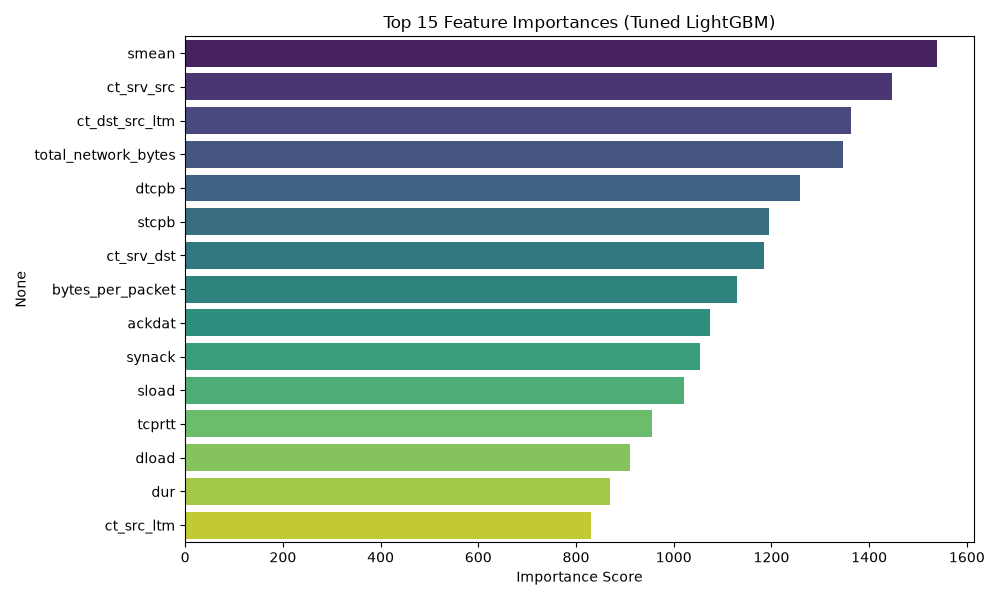
\includegraphics[width=0.9\textwidth]{figures/feature_importance.png}
    \end{columns}
\end{frame}

% Presenter: Kamal & François
\begin{frame}{Business \& Social Recommendation}
    \textbf{Deployment Recommendations for the CISO:}
    \vspace{0.3cm}
    \begin{itemize}
        \item \textbf{Automated Triage:} Deploy LightGBM as a front-line filter to automatically drop highly-malicious packets before they reach the core firewall.
        \item \textbf{Human-in-the-loop:} Maintain manual SOC review for edge-cases to prevent the NIDS from accidentally blocking critical business operations.
        \item \textbf{Ethical Considerations \& Bias:} The model was trained on a simulated environment. It may initially misclassify novel but benign IoT devices. We recommend continuous retraining to avoid discriminatory network throttling and combat "concept drift".
    \end{itemize}
\end{frame}

\begin{frame}
    \centering
    \Huge \textbf{Thank You!}
    
    \vspace{1cm}
    \Large Any Questions?
\end{frame}

\end{document}
